\documentclass{article}

%\usepackage{revtex4-1}
\usepackage{soul}
\usepackage{color}
\usepackage{outlines}
\usepackage{multirow}
\usepackage{array}
\usepackage{supertabular}
\usepackage{amsmath}
\usepackage[margin=1in]{geometry}
\usepackage{fancyhdr}
\usepackage{setspace}
\let\proof\relax
\let\endproof\relax
\usepackage{amsthm}
\usepackage{amssymb}
\usepackage{indentfirst}
%\usepackage{caption}
\pagestyle{headings}
\usepackage{setspace}
\usepackage[utf8]{inputenc}
%\usepackage[english]{babel}
\usepackage{graphicx}
\usepackage{textcomp}
\usepackage{gensymb}
\usepackage{url}
\usepackage{siunitx}
%\usepackage{subcaption}
\usepackage{float}
%\usepackage{circuitikz}
\usepackage{parskip}
\usepackage{wrapfig, lipsum, booktabs}
\usepackage{boldline}
\usepackage{pdfpages}
\usepackage{rotating}
\usepackage{tikz}
\usepackage[toc,page]{appendix}
\usepackage[colorlinks=false, linkbordercolor = {white}]{hyperref}
\usepackage{cases}
\usepackage{nomencl}
\usepackage{subcaption}
\usepackage{enumitem}
\usepackage{placeins}
\makenomenclature
\makeindex
%\newcommand{\cmmnt}[1]{\ignorespaces}
%\setlength{\belowcaptionskip}{-0.1in}

\title{Applications of Spline Interpolation to Solve ODE's}

%%% first author
\author{Andrew M. Chuen
%	\affiliation{
%		Student, 999099339\\
%		MAE 210 - Advanced Fluid Mechanics\\
%		Department of Mechanical Engineering\\
%		University of California\\
%		Davis, California 95616\\
%		Email: amchuen@ucdavis.edu
%	}	
}

\begin{document}
\maketitle
\section{Introduction}

Mathematical splines were originally introduced as a method to interpolate a set of points with lower-degree polynomials to avoid Runge's phenomenon. Cubic splines, in particular, were ideal not only due to computational efficiency with tridiagonal matrices, but also because they were low-order while still being able to account for inflection points within the intervals of interpolation. This can potentially be exploited to solve second order ODE's.

In this report, cubic spline interpolation is presented as a method to solve initial value problems. Section \ref{sec:algorithm} provides a general overview of the algorithm. Test case with which to evaluate the performance of the method are presented in section \ref{sec:testCases}. The results are shown and discussed in Sections \ref{sec:results} and \ref{sec:disc}, respectively.

\section{Cubic Spline Time-Stepping Algorithm}\label{sec:algorithm}

We start by assuming that a function $f(x)$ has continuous derivatives in the range $a\leq x \leq b$. The range is broken up into $n$ intervals through insertion of knot points $x_0, x_1,\dots,x_n$, where the knot points are unique ($a = x_0 < x_1 < \dots<x_n = b$). $s(x)$ is a cubic spline interpolating the function $f(x)$ if
\begin{enumerate}
	\item $s(x)$ is a cubic polynomial in each interval $\left[x_i, x_{i+1}\right]$
	\item $s(x_i) = f(x_i)$
	\item $s'(x)$ and $s''(x)$ are continuous
\end{enumerate}

The general formulation for a cubic spline function and its derivatives are given by the following:
\begin{align}
s_i(x) &= a_i + b_i(x-x_i)+c_i(x-x_i)^2 + d_i(x-x_i)^3\label{eqn:spline}\\
s'_i(x) &= b_i+2c_i(x-x_i) + 3d_i(x-x_i)^2\label{eqn:deriv}\\
s"_i(x) &= 2c_i + 6d_i(x-x_i)\label{eqn:deriv2}
\end{align}

Additionally, we will assume that $f(x)$ is governed by the general 2nd order ODE.
\begin{equation}
f'' + p(x)f' + q(x)f = r(x)\label{eqn:generic_ode}
\end{equation}
with initial conditions 
\begin{align*}
f(0) &= f_0\\
f'(0) &= f'_0
\end{align*}

Substituting equations (\ref{eqn:spline})-(\ref{eqn:deriv2}) into equation (\ref{eqn:generic_ode}) results in the following at each knot:
\begin{equation}
2c_i + p(x_i)b_i+q(x_i)a_i=r(x_i)\label{eqn:splineODE}
\end{equation}

When enforcing continuity between the $ith$ and $i+1th$ knots, equations (\ref{eqn:spline})-(\ref{eqn:deriv2}) and (\ref{eqn:splineODE}) form a system of equations from which the coefficients of the spline at $x_{i}$ can be obtained, assuming the function value and first and second derivatives at the $ith$ knot are known. Note the spacing $h_i$, is defined as $h_i = x_{i+1} - x_i$.
\begin{align}
a_{i+1} &= a_i + b_ih_i+c_ih_i^2 + d_ih_i^3\label{eqn:ai1}\\
b_{i+1} &= b_i+2c_ih_i + 3d_ih_i^2\label{eqn:bi1}\\
d_i &= \dfrac{c_{i+1} - c_i}{3h_i}\label{eqn:ci1}\\
c_{i+1} &= r(x_{i+1}) -  p(x_{i+1})b_{i+1} - q(x_{i+1})a_{i+1}\label{eqn:implicit}
\end{align}
Equation (\ref{eqn:implicit}) implicitly solves for the second derivative at the next knot. As such, iteration is needed at each step before the next time-step can be calculated. To start the iteration, an initial guess of 0 is assigned to $d_i$. In effect, this generates a quadratic spline that fits through the points at $x_i$ and $x_{i+1}$, allowing for $a_{i+1}$ and $b_{i+1}$ to be evaluated. These values are then passed into equation (\ref{eqn:implicit}) and updates the guess for $d_i$ in (\ref{eqn:ci1}). The process is repeated a few times at each step to ensure convergence.

\section{Test Cases}\label{sec:testCases}
Newton's Cannon and Eulerian rigid-body rotation are presented as the main test cases for this method. These cases were selected because the solutions for these problems are well known and provide a good benchmark to determine accuracy and performance of the method's implementation. Furthermore, because these problems are based in mechanics, conserved quantities such as energy can be evaluated to compare the method's performance.

\subsection{Newton's Cannonball}
Newton's cannonball describes the thought experiment presented by Isaac Newton hypothesizing the universal nature of gravitational force. This force determines the shape of the trajectories in the case of a two-body problem. Using Newton's second law and only accounting for gravitational force, the following non-dimensionalized system of ODE's are obtained.
\begin{align}
\ddot{x} + \omega^2 x &= 0\\
\ddot{y} + \omega^2 y &= 0
\end{align}
where $\omega^2$ describes the gravitational constant.
\begin{equation}
\omega^2 = \dfrac{\mu}{r^3} = \dfrac{\mu}{(x^2+y^2)^{(3/2)}}
\end{equation}
The gravity parameters, $\mu \in \left[0.4, 0.5, 0.6, 1\right]$, are used, which should recover hyperbolic, parabolic, elliptic, and circular orbits respectively. Additionally, energy and angular momentum will be calculated to ensure that the method is able to reproduce results without introducing noise into the system. The energy equation, $H$, is given by the following,
\begin{equation}
H = \dfrac{1}{2}\left[\dot{x}^2 + \dot{y}^2\right]-\left(x^2+y^2\right)^{-1/2}
\end{equation}

and the angular momentum equation is given by the following,
\begin{equation}
M = x\dot{y} - y\dot{x}
\end{equation}
For the purposes of the report, the time-scale considered is $t\in\left[0,50\right]$ with $\Delta t = 0.01$.
\subsection{Euler Equations for Rigid Body Rotation}
The Euler equations for rigid body rotation are given by the following.
\begin{equation}
\begin{split}
\dfrac{d^2\omega_1}{dt^2}+\beta\dfrac{d\omega_1}{dt}&=\alpha_1\omega_1\\
\dfrac{d^2\omega_2}{dt^2}+\beta\dfrac{d\omega_2}{dt}&=\alpha_2\omega_2\\
\dfrac{d^2\omega_3}{dt^2}+\beta\dfrac{d\omega_3}{dt}&=\alpha_3\omega_3
\end{split}
\end{equation}

where $\alpha_i$ is determined by the following
\begin{align}
\alpha_1 &= \omega^2_3\dfrac{(I_2 - I_3)(I_3 - I_1)}{I_1 I_2}+\omega^2_2\dfrac{(I_2 - I_3)(I_1 - I_2)}{I_1I_3}\\
\alpha_2 &= \omega^2_1\dfrac{(I_3 - I_1)(I_1 - I_2)}{I_2 I_3}+\omega^2_3\dfrac{(I_2 - I_3)(I_3 - I_1)}{I_2I_1}\\
\alpha_3 &= \omega^2_2\dfrac{(I_1 - I_2)(I_2 - I_3)}{I_3 I_1}+\omega^2_1\dfrac{(I_1 - I_2)(I_3 - I_1)}{I_3I_2}
\end{align}
and $I_1 = 3$, $I_2 = 2$, and $I_3 = 1$. Like the case of the Newton's cannon, the energy calculation is used to compare the performance of the spline time-stepping. The energy equation is given by the following,
\begin{equation}
E = \dfrac{1}{2}\left(\omega^2_1I_1+\omega^2_2I_2+\omega^2_3I_3\right)
\end{equation}
The initial conditions are given by the following, 
\begin{equation*}
\vec{\omega}(0) = \begin{bmatrix}
1\\0.01\\0.01
\end{bmatrix}\quad \dfrac{d\vec{\omega}}{dt}(0) = \vec{0}
\end{equation*}
and the time-scale considered is $t\in \left[0,80\right]$ with a time-step of $\Delta t = 0.016$.
\section{Results}\label{sec:results}
The results of the implementation are presented in this section. The method is compared to an explicit fourth-order Runge-Kutta method that uses the same interval size (note that the RK4 method computes intermediate values within each $\Delta t$ step-size). Figures \ref{fig:newtonSoln} and \ref{fig:eulerSoln} also show that the spline interpolation method is capable of generating an approximate solution to the problems presented in Section \ref{sec:testCases}.
\begin{figure}[H]
	\centering
	\begin{subfigure}{0.45\linewidth}
		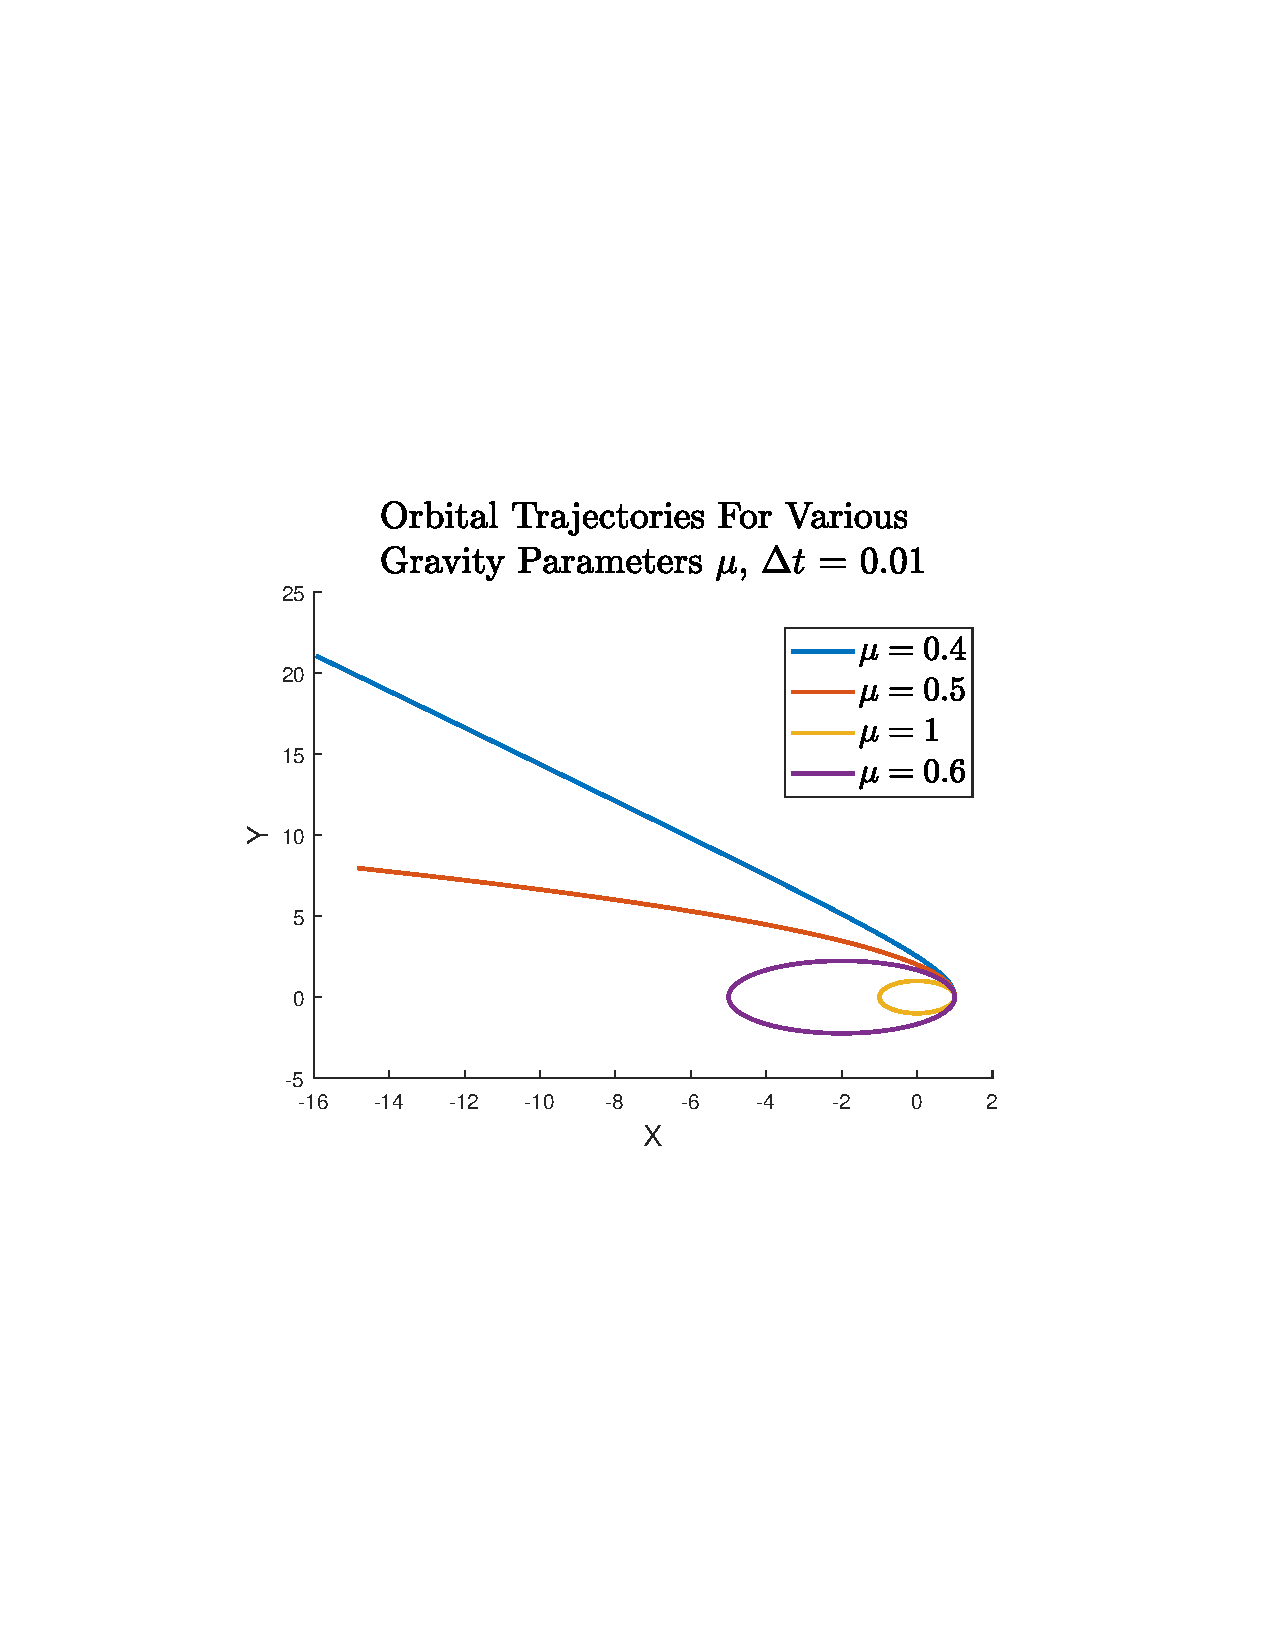
\includegraphics[trim={1.5in, 3in, 1.5in, 3in}, clip, width=\linewidth]{newtonOrbit}
		\caption{}\label{fig:newtonSoln}
	\end{subfigure}
	\begin{subfigure}{0.45\linewidth}
		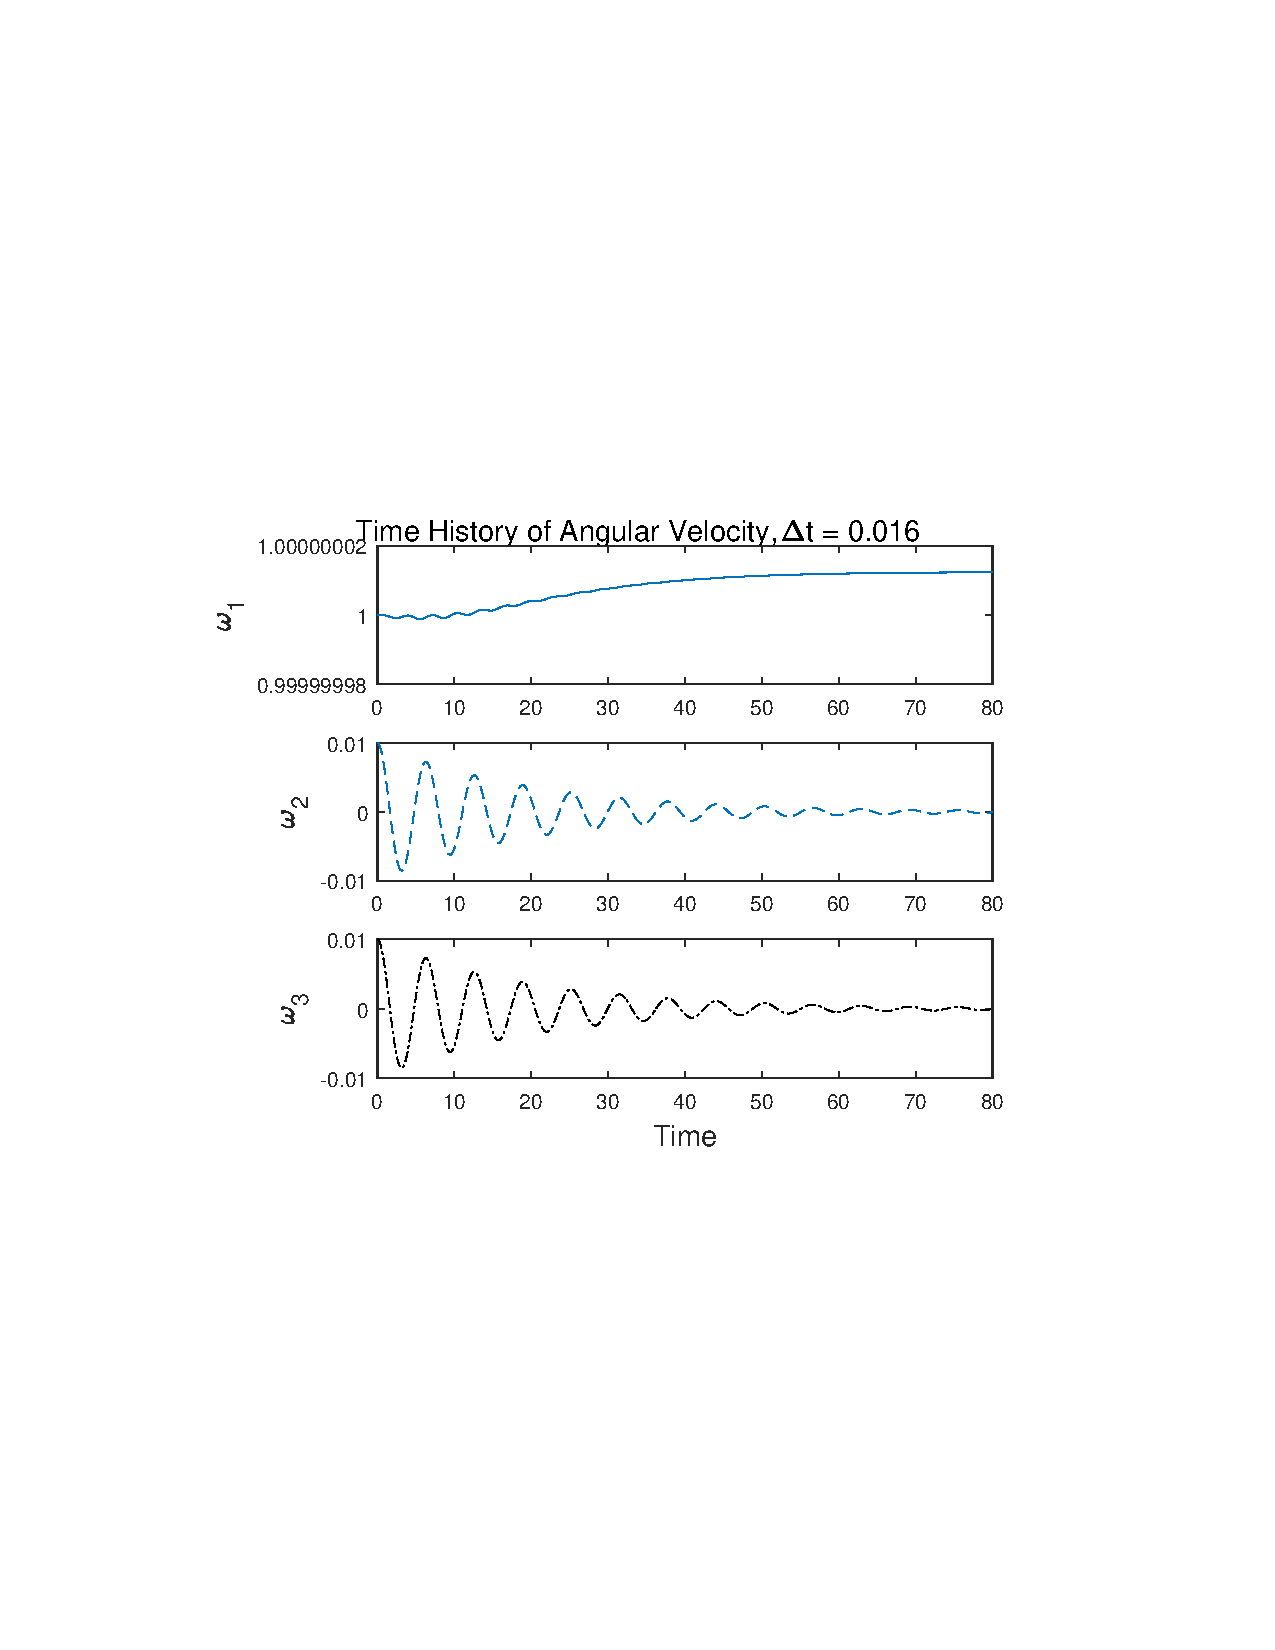
\includegraphics[trim={1.35in, 3in, 1.5in, 3in}, clip, width=\linewidth]{eulerSoln}
		\caption{}\label{fig:eulerSoln}
	\end{subfigure}
	\caption{Solutions to systems of equations presented in Section \ref{sec:testCases}.}
\end{figure} 

The following figures also show the performance of the cubic-spline method in solving the ODE's and calculating energy.
\begin{figure}[H]
\centering
\begin{subfigure}{0.45\linewidth}
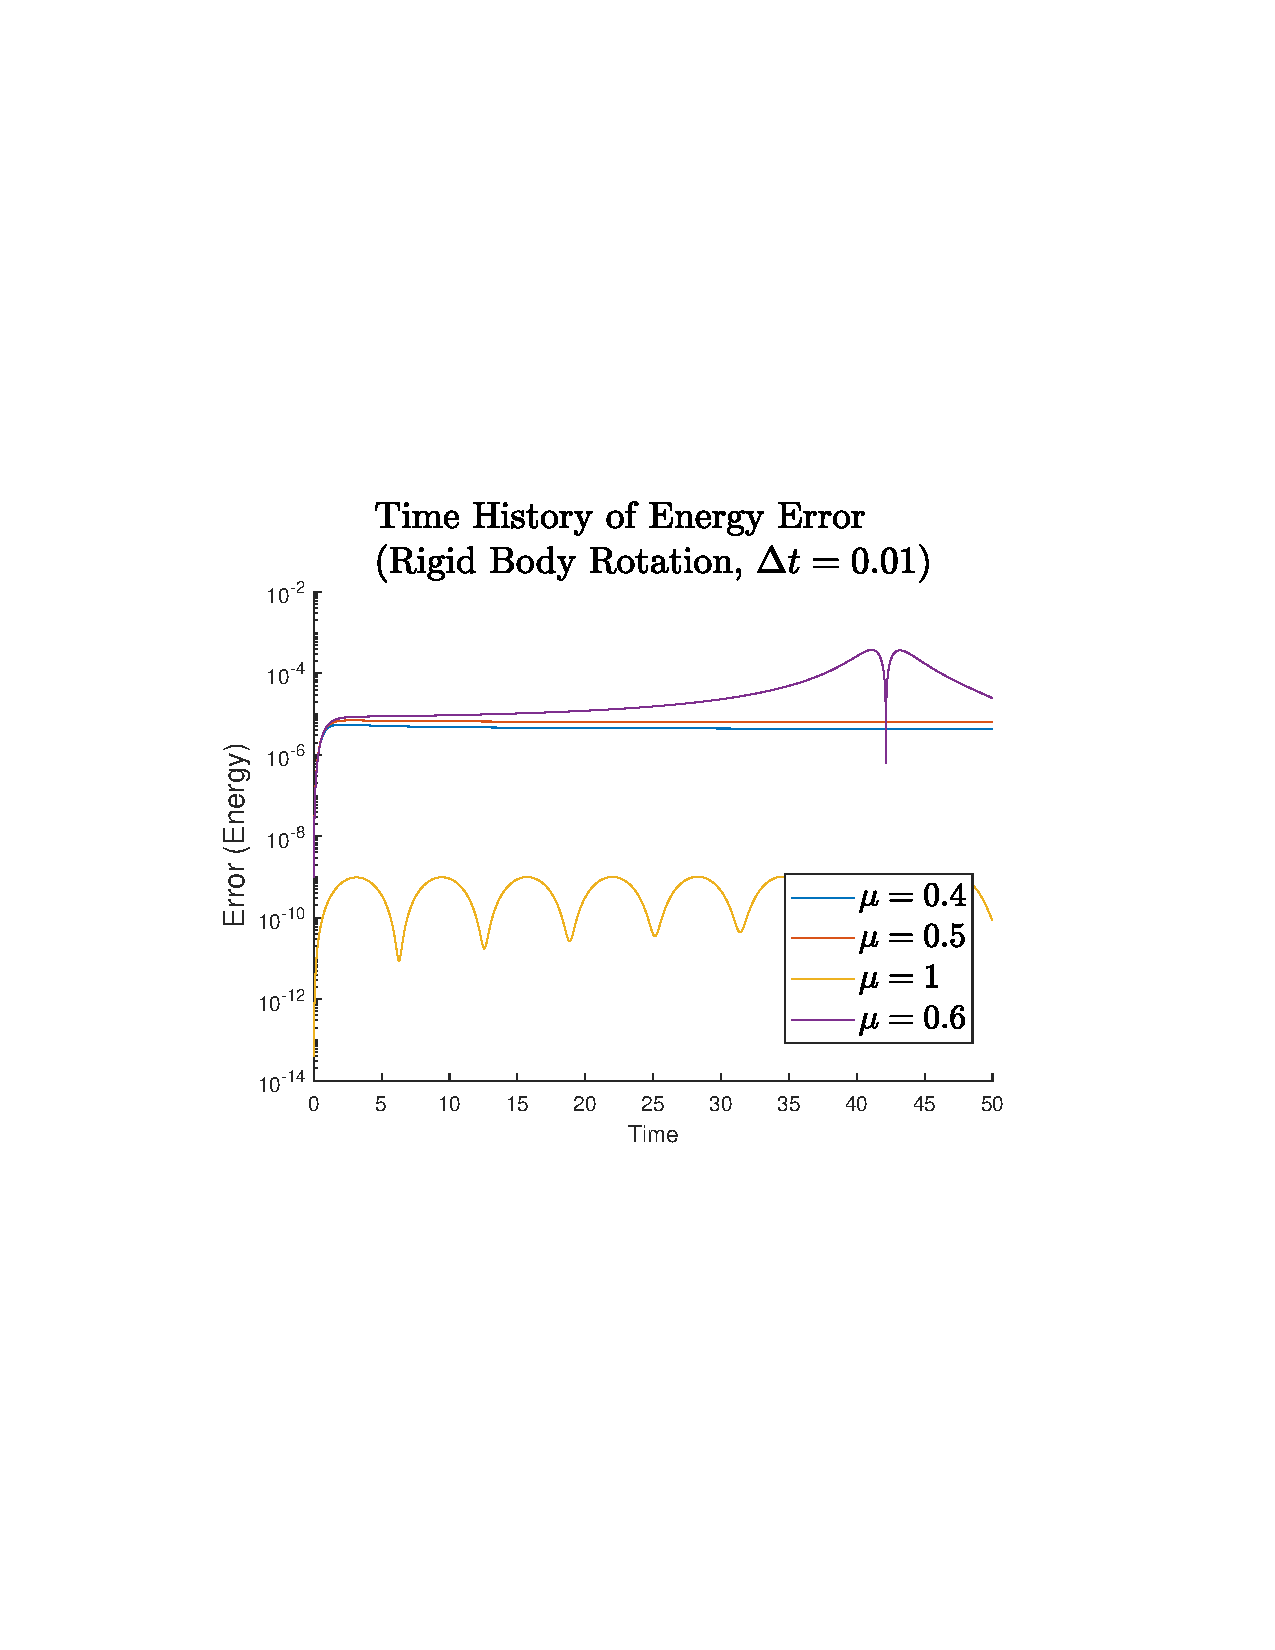
\includegraphics[trim={1.5in, 3in, 1.5in, 3in}, clip, width=0.95\linewidth]{newtonEnergyError}
\caption{}\label{fig:newtonEnergy}
\end{subfigure}
\begin{subfigure}{0.45\linewidth}
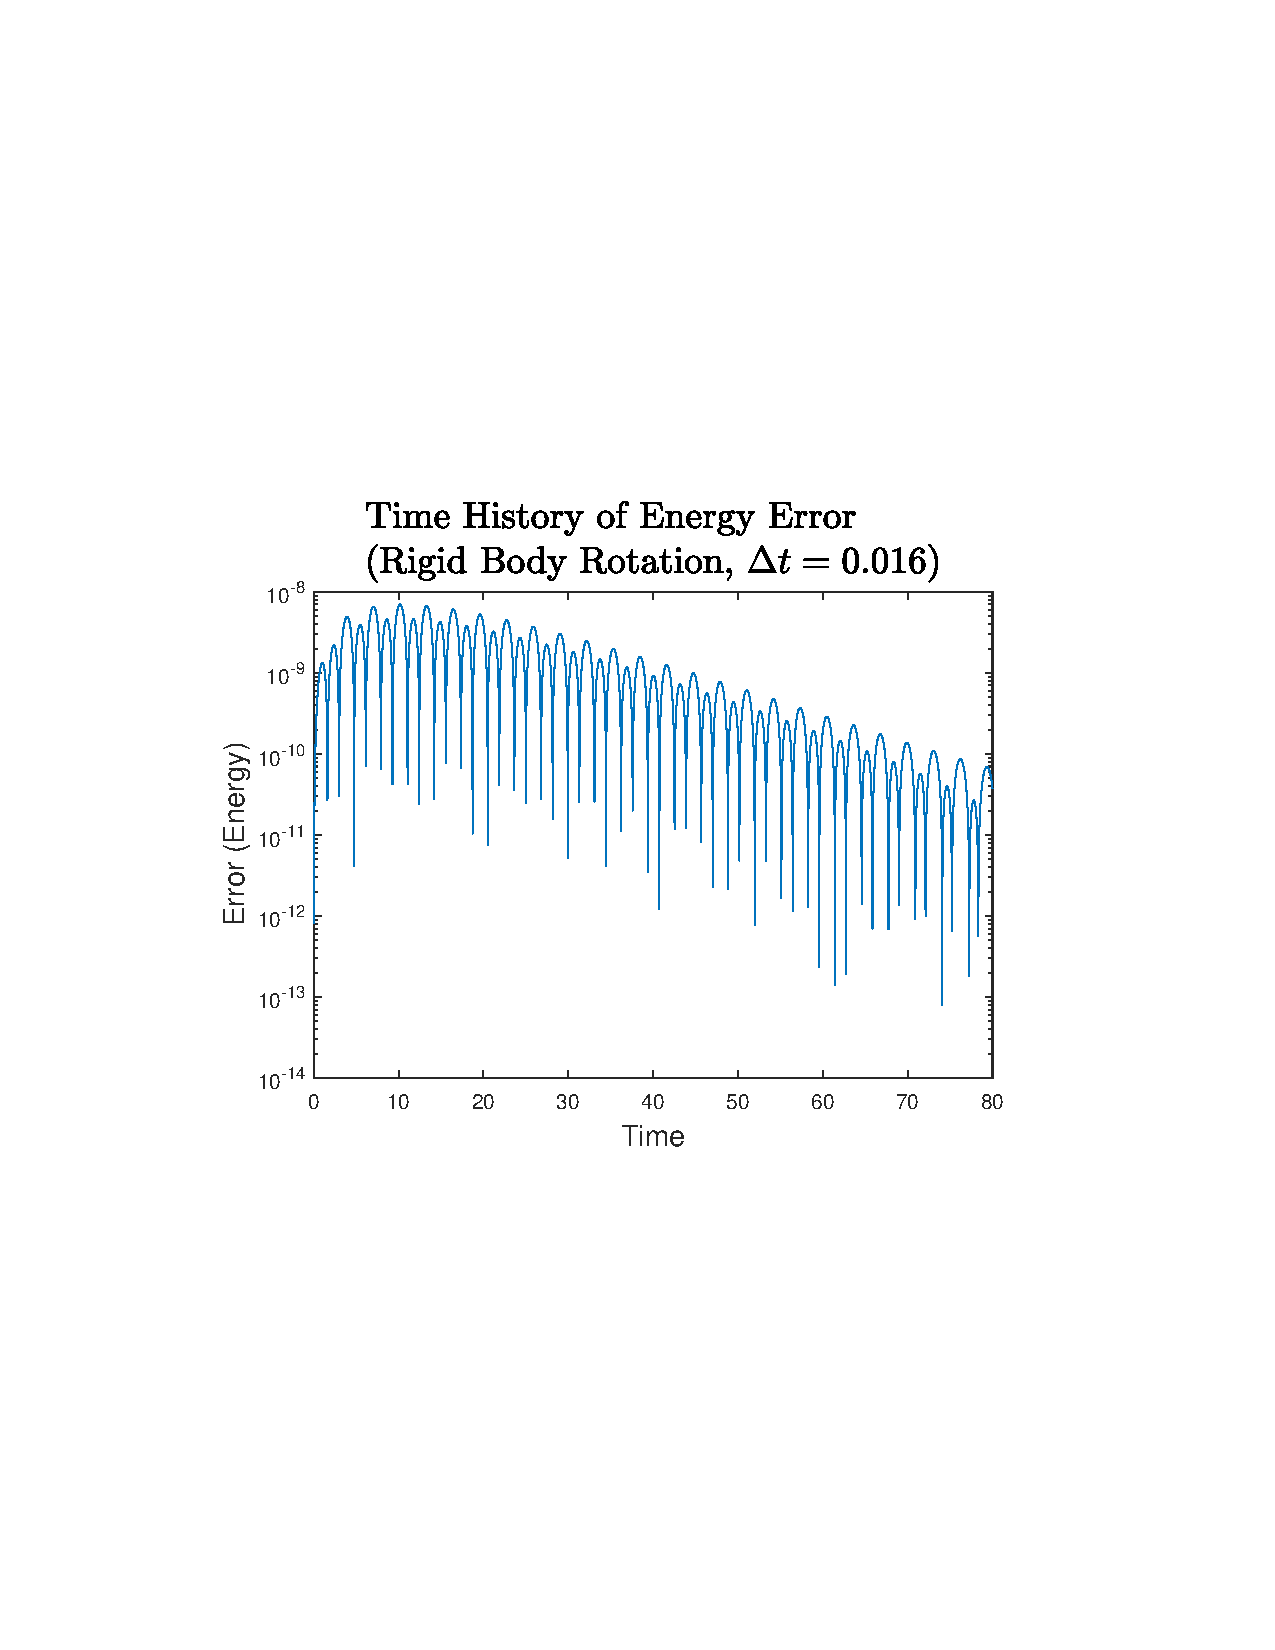
\includegraphics[trim={1.5in, 3in, 1.5in, 3in}, clip, width=0.95\linewidth]{eulerEnergyError}
\caption{}\label{fig:eulerEnergy}
\end{subfigure}
\caption{The plots above show the time-histories of the cubic spline's error performance.}
\end{figure} 
Figure \ref{fig:newtonConvergence} also shows the convergence behavior of cubic splines. In the case of Newton's Cannonball, it has second-order convergence.
\begin{figure}[H]
\centering
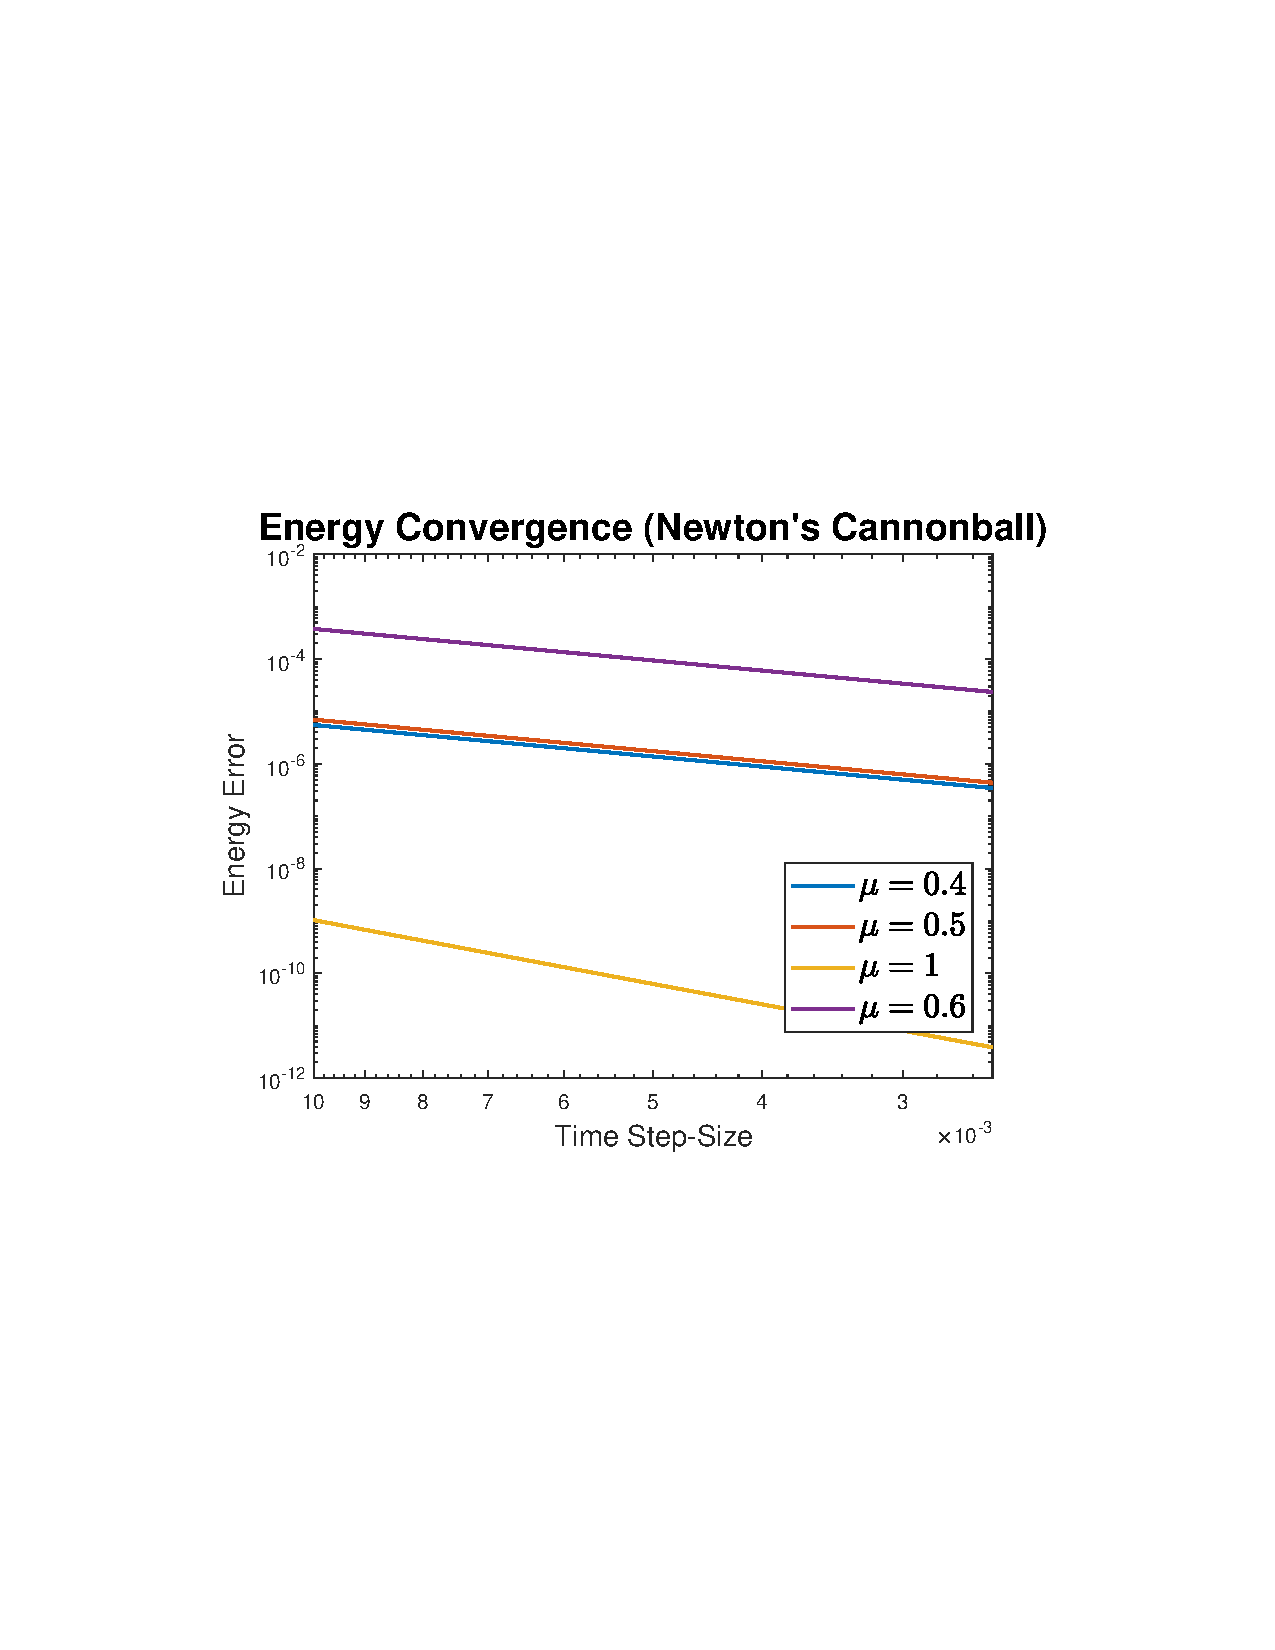
\includegraphics[trim={1.5in, 3in, 1.5in, 3in}, clip, width=0.45\linewidth]{newtonConvergence}
\caption{Convergence performance of cubic-spline in solving Newton's Cannonball.}\label{fig:newtonConvergence}
\end{figure}
\section{Discussion}\label{sec:disc}

% Discuss quality of result
Figures \ref{fig:newtonEnergy} and \ref{fig:eulerEnergy} show that the errors for the spline interpolation method are generally minimal, as they do not exceed $10^-3$. In the case of rigid-body rotation, the method performs quite well as it is able to calculate the result with a nominal tolerance. In the case of Newton's cannonball, however, the results exhibit unusual error corresponding with the trajectory of the orbit itself. It is likely that the spline is having more difficulty with proper calculations in regions with higher curvatures. Figure \ref{fig:newtonConvergence} shows that the cubic-spline does converge with smaller step-size, and it exhibits a second-order convergence rate. This shows that the method is stable and able to produce usable results.

% Discuss reason for oscillating error between this method and RK4

% Discuss possible options for improvement
Some possible directions to improve this method include improving the way values of $d_i$ and the coefficients at $x_{i+1}$ are calculated. There may be a way to feasibly obtain the coefficients at all points in a single sweep or set of iterations through the use of Newton's method and LU-decomposition. Additionally, it may be useful to consider obtaining improved accuracy through adaptability. Accumulation of errors could be a result of insufficient points to account for difficult curvatures in the function.

Using higher-order polynomial splines is another possible direction for improvement. Higher-order polynomials may provide the additional continuity of derivatives through the knots, which can improve the order of approximation of the spline and increase the convergence rate. 

A formal proof of its convergence may lend some insight into its performance and potential strategies to improve the method. 

\section{Conclusion}
Cubic splines are presented as a method to solve ordinary differential equations. The method utilizes iteration at every time-step to implicitly calculate the third derivative and the next time-step's coefficients. Using splines produces approximations that are capable of reaching desired tolerance levels with 2nd-order convergence. Further improvements will need to be made to make the method a viable solver.

\end{document}